\documentclass{article}
\usepackage[utf8]{inputenc}
\usepackage{amsmath}
\usepackage{amssymb}
\usepackage{babel}
\usepackage{graphicx}
\usepackage{pdfpages}

\graphicspath{{Images/}}

\setlength{\oddsidemargin}{0in}
\setlength{\textwidth}{6.5in}
\setlength{\topmargin}{-.55in}
\setlength{\textheight}{9in}
\pagestyle{empty}


\title{Solid State Physics HW2}
\author{Michael Nameika}
\date{September 2022}

\begin{document}

\maketitle

\section*{Problem 1}


The ionic radii for $\text{Zn}^{2+}$ and $\text{S}^{2-}$ are 0.074 and 0.026 nm respectively. Calculate the lattice parameter for the cubic structure of ZnS. 
\newline\newline

Recall that the cubic structure for ZnS is a face centered cubic structure of Zinc atoms with a face centered cubic structure of Sulfur atoms displaced by $(1/4,1/4,1/4)$. Then the nearest neighbor distance to an atom in the ZnS structure is given by 
\[d_{\text{nn}} = \frac{\sqrt{3}}{4}a\]
where $d_{\text{nn}}$ denotes the nearest neighbor distance and $a$ is the lattice parameter. Additionally, from the hard sphere model, we know that the nearest neighbor spheres touch at precisely one point. Then the center to center distance of two nearest neighbor spheres is given by
\[r_{\text{Zn}^{2+}} + r_{\text{S}^{2-}} = 0.074 \:\:\text{nm} + 0.026 \:\:\text{nm} = 0.100 \:\:\text{nm}\]
Notice that this is also the nearest neighbor distance. Then combining the above equation with the equation for $d_{\text{nn}}$, we find
\[\frac{\sqrt{3}}{4}a = 0.100 \:\: \text{nm}\]
Solving for a, we find
\[a = \frac{0.400 \:\: \text{nm}}{\sqrt{3}}\]
\[ \approx 0.231 \:\: \text{nm}\]
So our lattice parameter $a$ is approximately equal to $0.231 \:\: \text{nm}$.
\newline\newline

\section*{Problem  2}


A beam of electrons ($I = 20 \: \text{mA}$) hits the anode in the X-ray source. The electrons are accelerated by the 40 kV potential difference. That is, each electron has 40 keV energy. Determine the number of X-ray photons generated by the collision per second. For simplicity, assume that each photon has a wavelength of $1 \: \text{\AA}$, (0.1 nm).
\newline

Recall that $1 \text{ A} = 1 \frac{\text{c}}{s}$ and that the electron has a charge of $1.602 \times 10^{-19} \: \text{c}$. We first wish to find the number of electrons per second in the beam of $20 \: \text{mA}$. Well, to do so, we must divide the current of the beam by the charge of the electron. Let $n_e$ denote the number of electrons per second. Then
\[n_e = \frac{2.000 \times 10^{-2} \: \text{c/s}}{1.602 \times 10^{-19} \: \text{c}} \approx 1.248 \times 10^{17} \: \frac{\text{electrons}}{s}\]
We are given the wavelength of each X-ray is $1 \: \text{\AA}$, so we may calculate the energy of each X-ray by the following formula:
\[\lambda = \frac{12.4 \: \text{\AA}}{E \: (\text{keV})}\]
Solving, it is clear to see that the energy of each X-ray is $1.24 \times 10^3 \: \text{eV}$. Now, each electron has an energy 40 keV, so assuming elastic scattering, we may calculate how many X-rays are generated per electron by dividing the electron energy by the X-ray energy:
\[\frac{4 \times 10^4 \: \text{keV}}{1.24 \times 10^3 \: \text{eV}} \approx 32.3 \: \frac{\text{X-rays}}{\text{electron}}\]
Now, we can find the number of X-rays generated per second by multiplying the above equation by how many electrons are being generated per second. Doing so gives us the following:
\[\left(32.3 \: \frac{\text{X-rays}}{\text{electron}}\right)\left(1.248 \times 10^{17} \: \frac{\text{electrons}}{s}\right)\]
\[ \approx 4.03 \times 10^{18} \frac{\text{X-rays}}{s}\]



\section*{Problem 3}

Assuming that like ions do not touch in either the NaCl or CsCl structures, calculate the relative packing efficiencies of both structures, for example as a function of $r_c/r_a$. Verify the result for the limit where the sizes of the cations and anions become the same.
\newline

Recall that NaCl is face centered cubic crystal structure. Then there will be four NaCl molecules per unit cell. Recall the formula for packing efficiency of a crystal:
\[PE (\text{packing efficiency}) = \frac{\text{( \# of atoms)(volume per atom)}}{V_c}\]
where $V_c$ denotes the volume of the cell. Additionally, notice that the lattice parameter $a$ is given by $a = 2r_a + 2r_c$ since NaCl is an fcc lattice with an interlaced fcc latice displaced by (1/2, 0, 0), so the nearest neighbor distance is $a/2$ which is equal to $r_a + r_c$ using the hard ball model. Now, since there are four NaCl molecules per unit cell, we find
\[PE_{\text{NaCl}} = \frac{4(4\pi/3)r_c^3 + 4(4\pi/3)r_a^3}{(2r_c + 2r_a)^3}\]
\[ = \frac{2\pi}{3}\frac{r_c^3 + r_a^3}{(r_c + r_a)^3}\]
and writing as a function of $r_c/r_a$:
\[PE_{\text{NaCl}} = \frac{2\pi}{3}\frac{1 + \left(\frac{r_c}{r_a}\right)^3}{\left(1 + \frac{r_c}{r_a}\right)^3}\]
Now, we wish to verify that this formula is consistent when we allow for the maximum possible size of $r_c$ and the maximum possible size of $r_a$. Consider first the case where we allow the maximum possible size of $r_a$:
\begin{center}
    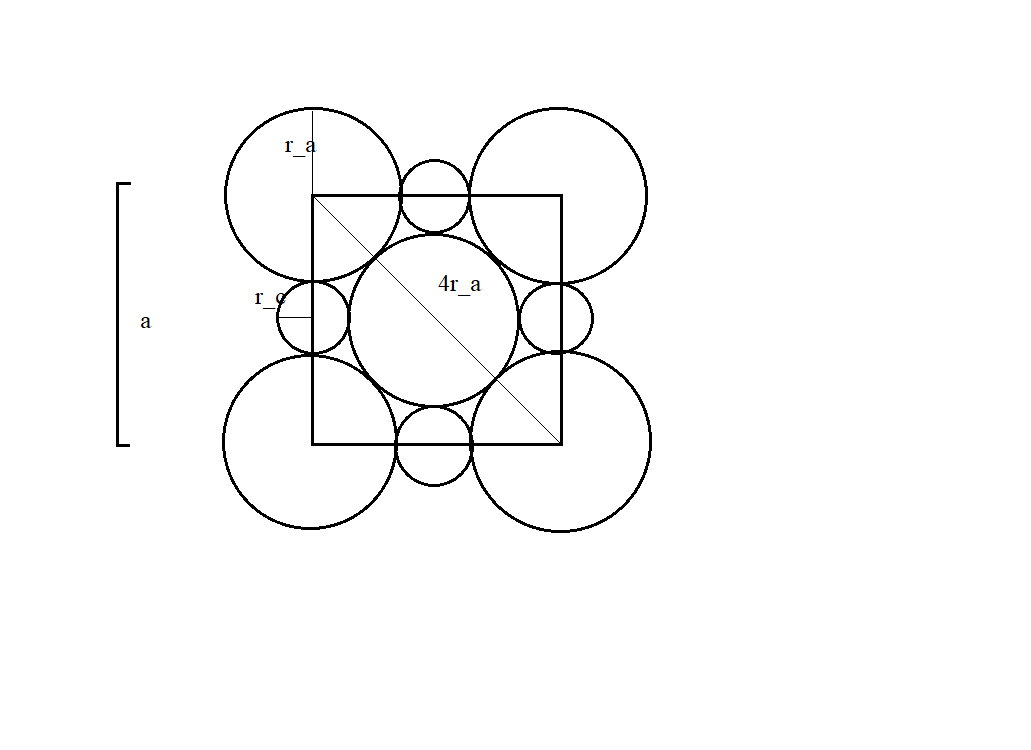
\includegraphics[scale = 0.4]{NaClraLim.png}
\end{center}


Notice from the above figure that $4r_a = \sqrt{2}a$ and so $2\sqrt{2}r_a = a$. Using the fact that $a = 2r_c + 2r_a$, we may solve for $r_c$:
\[a = 2r_c + 2r_a = 2\sqrt{2}r_a\]
\[2r_c = (2\sqrt{2} - 2)r_a\]
\[r_c = (\sqrt{2} - 1)r_a\]
And plugging this into the equation we found for the packing efficiency, we find
\[PE_{r_a} = \frac{2\pi}{3}\frac{1 + (\sqrt{2} - 1)^3}{(1 + \sqrt{2} - 1)^3}\]

Now, for the case where we allow the size of $r_c$ to reach its maximum possible size:
\begin{center}
    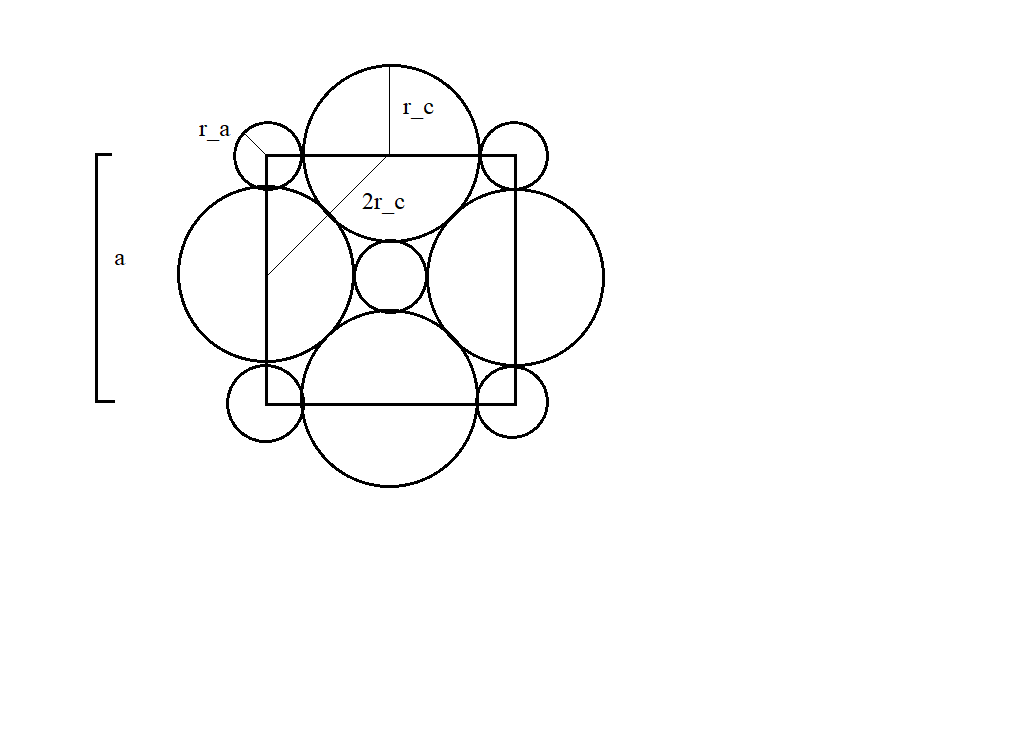
\includegraphics[scale = 0.4]{NaClrcLim.png}
\end{center}
Notice from the above figure that $2r_c = \frac{a}{\sqrt{2}}$ and so solving for $r_a$, we find
\[2r_a + 2r_c = 2\sqrt{2}r_c\]
\[2r_a = (2\sqrt{2} - 2)r_c\]
\[r_a = (\sqrt{2} - 1)r_c\]
Plugging this into the equation we found for the packing efficiency, we find
\[PE = \frac{2\pi}{3}\frac{1 + \left(\frac{1}{\sqrt{2} - 1}\right)^3}{\left(1 + \frac{1}{\sqrt{2}-1}\right)^3}\]
Multiplying the top and bottom by $(\sqrt{2}-1)^3$, we find
\[PE_{r_c} = \frac{2\pi}{3}\frac{(\sqrt{2}-1)^3 + 1}{(\sqrt{2} - 1 + 1)^3}\]
\[ = PE_{r_a}\]
which evaluates to 
\[PE \approx 0.793\]
Now we must calculate the packing efficiency for CsCl.
\newline


For CsCl, the crystal structure is simple cubic with an additional simple cubic lattice displaced by (1/2,1/2,1/2) and so has 1 anion and 1 cation per unit cell. Additionally, notice that $a = \frac{2}{\sqrt{3}}(r_a + r_c)$. Then the formula for packing efficiency for CsCl is
\[PE_{\text{CsCl}} = \frac{(4\pi/3r_a^3) + (4\pi/3r_c^3)}{(2/\sqrt{3}(r_a + r_c))^3}\]
\[ = \frac{\sqrt{3}\pi}{2} \frac{r_a^3 + r_c^3}{(r_a + r_c)^3}\]
Writing as a function of $r_c/r_a$:
\[PE_{\text{CsCl}} = \frac{\sqrt{3}\pi}{2} \frac{1 + \left(\frac{r_c}{r_a}\right)^3}{(1 + \frac{r_c}{r_a})^3}\]
Now we must verify for the case where we maximize $r_c$:

\begin{center}
    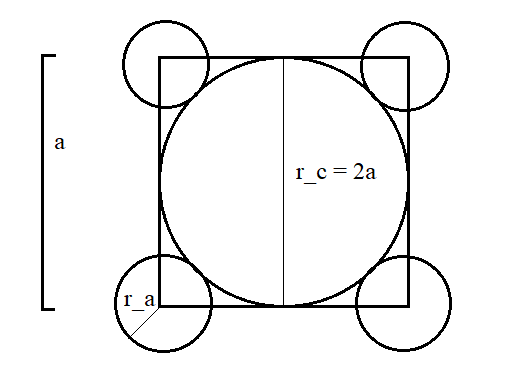
\includegraphics[scale = 0.4]{CsClrcLim.PNG}
\end{center}

From the above figure, notice that $a = 2r_c$. Now we may calculate $r_a$ given $a = \frac{2}{\sqrt{3}}(r_a + r_c)$:

\[a = \frac{2}{\sqrt{3}}(r_a + r_c) = 2r_c\]
\[\frac{2}{\sqrt{3}}r_a = (2 - \frac{2}{\sqrt{3}})r_c\]
so
\[r_c = \frac{1}{\sqrt{3}-1}r_a\]
Now, plugging this into the equation we found the packing efficiency, we find
\[PE_{r_c} = \frac{\sqrt{3}\pi}{2} \frac{1 + \left(\frac{1}{\sqrt{3}-1}\right)^3}{\left(1 + \frac{1}{\sqrt{3}-1}\right)^3}\]
And multiplying the top and bottom by $(\sqrt{3} - 1)^3$, we find
\[PE_{r_c} = \frac{\sqrt{3}\pi}{2} \frac{(\sqrt{3} - 1)^3 + 1}{(\sqrt{3})^3}\]
Now, in the limit where $r_a$ is allowed to its maximum size, we find $a = 2r_a$, as in the figure below.

\begin{center}
    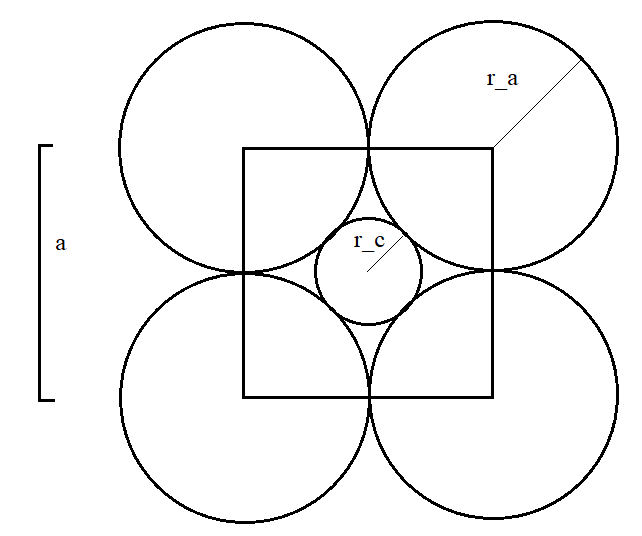
\includegraphics[scale = 0.5]{CsClraLim.PNG}
\end{center}
Solving for $r_c$, we find
\[a = \frac{2}{\sqrt{3}}(r_a + r_c) = 2r_a\]
\[r_c = (\sqrt{3}-1)r_a\]
and substituting this into the equation we found for packing efficiency, we find
\[PE_{r_a} = \frac{\sqrt{3}\pi}{2} \frac{(\sqrt{3}-1)^3 + 1}{(\sqrt{3})^3}\]
\[= PE_{r_c}\]
and 
\[PE_{r_a} \approx 0.729\]


\section*{Problem 4}


\textbf{\textit{Hexagonal space lattice.}}  The primitive translation vectors of the hexagonal space lattice may be taken as 
\[\textbf{a}_1 = \frac{\sqrt{3}a}{2}\hat{\textbf{{x}}} + \frac{a}{2}\hat{\textbf{y}} \:\:\: ; \:\:\:\:\:\:\:\:\: \textbf{a}_2 = -\frac{\sqrt{3}a}{2}\hat{\textbf{x}} + \frac{a}{2}\hat{\textbf{y}} \:\:\: ; \:\:\:\:\:\:\:\:\: \textbf{a}_3 = c\hat{\textbf{z}}\]

(a) Show that the volume of the primitive cell is $\frac{\sqrt{3}}{2}a^2c$.
\newline

Proof: Recall that the volume of a solid in $\mathbb{R}^3$ generated by three linearly independent vectors $\textbf{a}_1, \textbf{a}_2, \textbf{a}_3$ is given by
\[V = \textbf{a}_1 \cdot (\textbf{a}_2 \times \textbf{a}_3)\]
Using the basis vectors given at the beginning of the problem, we find
\[V_{hl} = \left( \frac{\sqrt{3}a}{2}\hat{\textbf{x}} + \frac{a}{2}\hat{\textbf{y}} \right) \cdot \left(\left[ -\frac{\sqrt{3}a}{2} \hat{\textbf{x}} + \frac{a}{2} \hat{\textbf{y}} \right] \times \left[ c \hat{\textbf{z}} \right]\right)\]
Where $V_{hl}$ denotes the volume of the hexagonal lattice. Simplifying the cross product in the above expression, we find
\[V_{hl} = \left( \frac{\sqrt{3}a}{2}\hat{\textbf{x}} + \frac{a}{2} \hat{\textbf{y}} \right) \cdot \left( \frac{ac}{2}\hat{\textbf{x}} + \frac{\sqrt{3}ac}{2} \hat{\textbf{y}} \right)\]
which further simplifies to
\[V_{hl} = \frac{\sqrt{3}}{2}a^2c\]
which is what we wished to show.
\newline

(b) Show that the primitive translations of the reciprocal lattice are
\[\textbf{b}_1 = \frac{2\pi}{\sqrt{3}a}\hat{\textbf{x}} + \frac{2\pi}{a}\hat{\textbf{y}} \:\:\: ; \:\:\:\:\:\:\: \textbf{b}_2 = -\frac{2\pi}{\sqrt{3}a} \hat{\textbf{x}} + \frac{2\pi}{a} \hat{\textbf{y}} \:\:\: ; \:\:\:\:\:\:\: \textbf{b}_3 = \frac{2\pi}{c} \hat{\textbf{z}}\]

Proof: From part (a), we showed that $V_c = \frac{\sqrt{3}}{2}a^2c$, and $\textbf{a}_2 \times \textbf{a}_3 = \frac{ac}{2}\hat{\textbf{x}} + \frac{\sqrt{3}ac}{2}\hat{\textbf{y}}$. Using these results, it is immediately clear that $\textbf{b}_1$ can be written as
\[\textbf{b}_1 = 2\pi \frac{ac/2 \hat{\textbf{x}} + \sqrt{3}/2ac\hat{\textbf{y}}}{\sqrt{3}/2a^2c} = \frac{2\pi}{\sqrt{3}a}\hat{\textbf{x}} + \frac{2\pi}{a}\hat{\textbf{y}}\]
Now, for $\textbf{b}_2$, we must first calculate $\textbf{a}_3 \times \textbf{a}_1$:
\[\textbf{a}_3 \times \textbf{a}_1 = (c\hat{\textbf{z}}) \times \left( \frac{\sqrt{3}a}{2} \hat{\textbf{x}} + \frac{a}{2}\hat{\textbf{y}} \right) = -\frac{ac}{2}\hat{\textbf{x}} + \frac{\sqrt{3}ac}{2}\hat{\textbf{y}}\]
Then 
\[\textbf{b}_2 = 2\pi \frac{-ac/2 \hat{\textbf{x}} + \sqrt{3}/2ac\hat{\textbf{y}}}{\sqrt{3}{2}a^2c}\]
which simplifies to
\[\textbf{b}_2 = -\frac{2\pi}{\sqrt{3}a}\hat{\textbf{x}} + \frac{2\pi}{a}\hat{\textbf{y}}\]
Finally, for $\textbf{b}_3$, we must compute $\textbf{a}_1 \times \textbf{a}_2$:
\[\textbf{a}_1 \times \textbf{a}_2 = \left( \frac{\sqrt{3}a}{2}\hat{\textbf{x}} + \frac{a}{2} \hat{\textbf{y}} \right) \times \left( -\frac{\sqrt{3}a}{2}\hat{\textbf{x}} + \frac{a}{2}\hat{\textbf{y}} \right)\]
\[ = \frac{\sqrt{3}a^2}{2} \hat{\textbf{z}}\]
And evaluating for $\textbf{b}_3$:
\[\textbf{b}_3 = 2\pi \frac{\sqrt{3}a^2/2 \hat{\textbf{z}}}{\sqrt{3}/2a^2c} = \frac{2\pi}{c}\hat{\textbf{z}}\]
Finally, we found $\textbf{b}_1, \textbf{b}_2, \textbf{b}_3$ to be defined by
\[\textbf{b}_1 = \frac{2\pi}{\sqrt{3}a}\hat{\textbf{x}} + \frac{2\pi}{a}\hat{\textbf{y}} \:\:\: ; \:\:\:\:\:\:\: \textbf{b}_2 = -\frac{2\pi}{\sqrt{3}a}\hat{\textbf{x}} + \frac{2\pi}{a}\hat{\textbf{y}} \:\:\: ; \:\:\:\:\:\:\: \textbf{b}_3 = \frac{2\pi}{c}\hat{\textbf{z}}\]
which is precisely what we sought to show.
\newline

(c) Describe and sketch the first Brillouin zone of the hexagonal space lattice.
\newline

The first Brillouin zone of the hexagonal space lattice is also a hexagonal space lattice. 
To see this, notice that $\textbf{b}_1 \cdot \textbf{b}_3 = \textbf{b}_2 \cdot \textbf{b}_3 = 0$. That is, $\textbf{b}_3$ is orthogonal to both $\textbf{b}_1$ and $\textbf{b}_2$. Additionally, we will show that the angle between $\textbf{b}_1$ and $\textbf{b}_2$ is $60^{\circ}$ and $||\textbf{b}_1|| = ||\textbf{b}_2||$.
\newline
Notice
\[||\textbf{b}_1|| = \sqrt{ \left(\frac{2\pi}{\sqrt{3}a}\right)^2 + \left( \frac{2\pi}{a} \right)^2} = \sqrt{4\pi^2\left( \frac{4}{3a^2} \right)} = \frac{2\pi}{\sqrt{3}a}\]
\[||\textbf{b}_2|| = \sqrt{\left(-\frac{2\pi}{\sqrt{3}a}\right)^2 + \left( \frac{2\pi}{a} \right)^2} = \sqrt{4\pi^2\left( \frac{4}{3a^2} \right)} = \frac{2\pi}{\sqrt{3}a} = ||\textbf{b}_1||\]
Now, recall that the angle between two vectors is given by
\[\theta = \arccos{\left( \frac{\textbf{b}_1 \cdot \textbf{b}_2}{||\textbf{b}_1||||\textbf{b}_2||} \right)}\]
Next, let's find $\textbf{b}_1 \cdot \textbf{b}_2$:
\[\textbf{b}_1 \cdot \textbf{b}_2 = \left( \frac{2\pi}{\sqrt{3}a}\hat{\textbf{x}} + \frac{2\pi}{a}\hat{\textbf{y}} \right) \cdot \left( -\frac{2\pi}{\sqrt{3}a}\hat{\textbf{x}} + \frac{2\pi}{a}\hat{\textbf{y}} \right) = \frac{4\pi^2}{a^2} \left( -\frac{1}{3} + 1 \right) = \frac{8\pi^2}{3a^2}\]
Plugging these equations into the equation for $\theta$, we find
\[\theta = \arccos{\left( \frac{8\pi^2/(3a^2)}{16\pi^2/(3a^2)} \right)} = \arccos{\left( \frac{1}{2} \right)} = \frac{\pi}{6} = 60^{\circ}\]
So the angle between $||\textbf{b}_1||$ and $||\textbf{b}_2||$ is $60^{\circ}$. Putting it all together, we have
\begin{align*}
    b_1 = b_2 \neq b_3\\
    \alpha = \beta = 90^{\circ}\\
    \gamma = 60^{\circ}\\
\end{align*}
which defines a hexagonal lattice. See attached for sketch.

\section*{Problem 5}


\textbf{\textit{Volume of Brillouin zone.}} Show that the volume of the first Brillouin zone is $(2 \pi)^3/V_c$, where $V_c$ is the volume of a crystal primitive cell. 
\newline

Proof: Similar to problem 4, we may find find $V_B$, the volume of the first Brillouin zone, by the following equation:
\begin{equation}
    V_B = \textbf{b}_1 \cdot (\textbf{b}_2 \times \textbf{b}_3)
\end{equation}

where $\textbf{b}_1, \textbf{b}_2, \textbf{b}_3$ are the basis vectors for the reciprocal space. 
\newline
To begin, recall the formulas for the basis vectors in the reciprocal space:
\begin{equation}
    \textbf{b}_1 = 2\pi \frac{\textbf{a}_2 \times \textbf{a}_3}{\textbf{a}_1 \cdot ( \textbf{a}_2 \times \textbf{a}_3)}, \:\:\:\: \textbf{b}_2 = 2\pi \frac{\textbf{a}_3 \times \textbf{a}_1}{\textbf{a}_1 \cdot ( \textbf{a}_2 \times \textbf{a}_3)}, \:\:\:\: \textbf{b}_3 = 2\pi \frac{\textbf{a}_1 \times \textbf{a}_2}{\textbf{a}_1 \cdot ( \textbf{a}_2 \times \textbf{a}_3)}
\end{equation}
Recall also that $\textbf{a}_1 \mathbf{\cdot} (\textbf{a}_2 \times \textbf{a}_3) = V_c$. Then plugging in (2) into (1) and substituting for $V_c$, we find
\[V_B = \frac{(2\pi)^3}{V_c^3}\left[ (\textbf{a}_2 \times \textbf{a}_3) \mathbf{\cdot} ((\textbf{a}_3 \times \textbf{a}_1) \times (\textbf{a}_3 \times \textbf{a}_2)) \right]\]
and using the identity $(\textbf{c} \times \textbf{a}) \times (\textbf{a} \times \textbf{b}) = (\textbf{c} \cdot (\textbf{a} \times \textbf{b})) 
\textbf{a}$, we find
\[V_B = \frac{(2\pi)^3}{V_c^3}\left[(\textbf{a}_2 \times \textbf{a}_3) \cdot (\textbf{a}_3 \cdot (\textbf{a}_1 \times \textbf{a}_3)) \textbf{a}_1 \right]\]
Rearranging terms, we can write the above equation as:
\begin{equation}
    V_B = \frac{(2\pi)^3}{V_c^3}\left[ (\textbf{a}_3 \cdot (\textbf{a}_1 \times \textbf{a}_2)(\textbf{a}_1 \cdot (\textbf{a}_2 \times \textbf{a}_3)) \right]
\end{equation}
Notice that $\textbf{a}_3 \cdot (\textbf{a}_1 \times \textbf{a}_2) = \textbf{a}_1 \cdot (\textbf{a}_2 \times \textbf{a}_3) = V_c$, so (3) simplifies as
\[V_B = \frac{(2\pi)^3}{V_c^3}(V_c^2)\]
\[V_B = \frac{(2\pi)^3}{V_c}\]
which is what we wanted to show.


\newpage
\section*{Hexagonal Reciprocal Space Sketch}

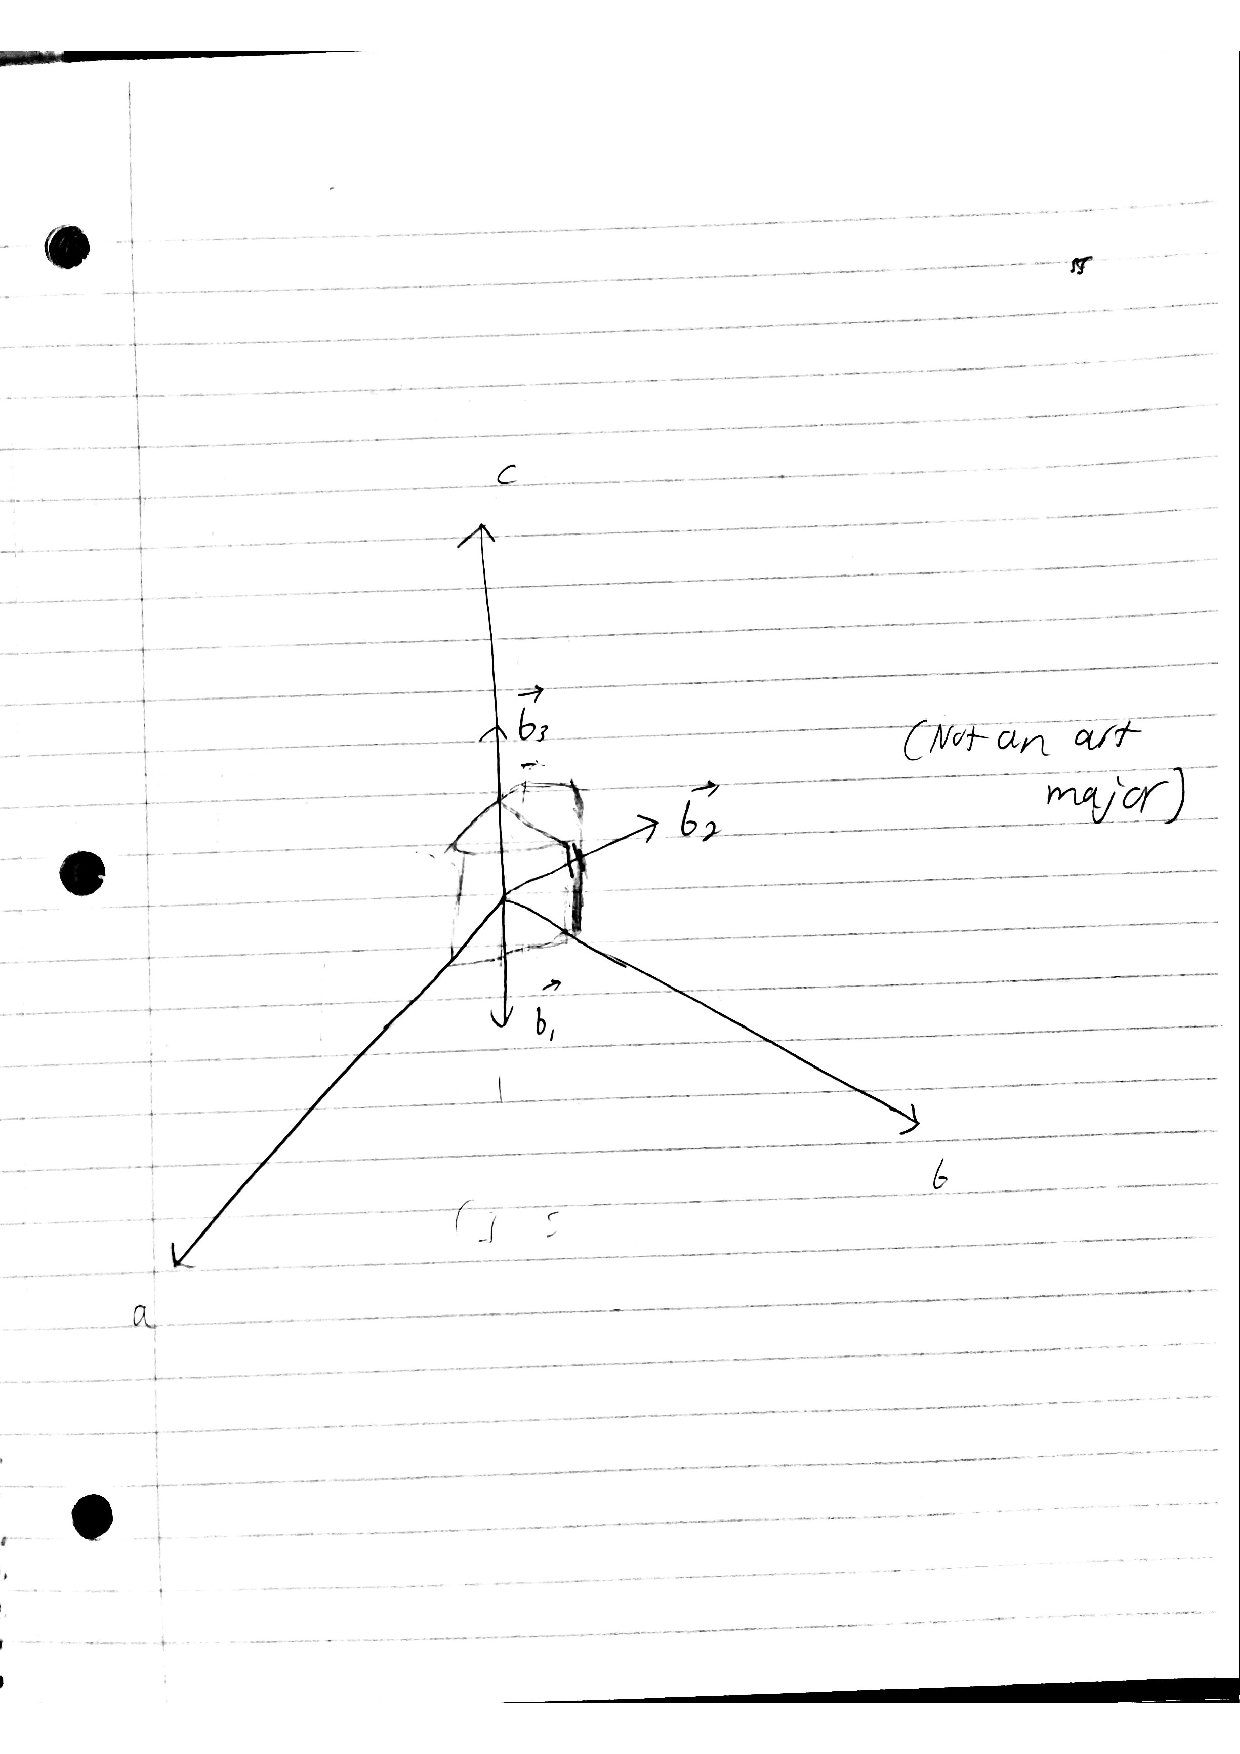
\includegraphics[scale = 0.75]{reciprocal sketch.pdf}


\end{document}
